\documentclass{article}
\usepackage[paperwidth=360pt,paperheight=275pt,margin=0pt,noheadfoot]{geometry}
\usepackage{tikz}
\usetikzlibrary{calc}

\definecolor{ink}{RGB}{28,41,56}
\definecolor{axis}{RGB}{100,116,139}
\definecolor{grid}{RGB}{203,213,225}
\definecolor{curve}{RGB}{30,64,175}
\definecolor{teal}{RGB}{13,148,136}
\definecolor{tealfill}{RGB}{176,227,219}
% Integral diagrams have one consistent three-colour vocabulary: blue for an
% under-only part, yellow for an over-only (or still-unresolved) part, and
% green for their common part.  The common part is explicit rather than an
% alpha blend, so it remains visibly distinct after GIF palette quantization.
\definecolor{cyan}{RGB}{0,84,134}
\definecolor{cyanfill}{RGB}{0,114,178}
\definecolor{yellow}{RGB}{184,134,11}
\definecolor{yellowfill}{RGB}{240,228,66}
\definecolor{overlap}{RGB}{15,110,67}
\definecolor{overlapfill}{RGB}{20,153,92}
\definecolor{orange}{RGB}{234,88,12}
\definecolor{orangefill}{RGB}{254,215,170}
\definecolor{purple}{RGB}{126,34,206}
\definecolor{yellowedge}{RGB}{202,138,4}
\definecolor{projection}{RGB}{148,163,184}
\colorlet{under}{cyan}
\colorlet{underfill}{cyanfill}
\colorlet{over}{yellow}
\colorlet{overfill}{yellowfill}
\colorlet{shared}{overlap}
\colorlet{sharedfill}{overlapfill}
\colorlet{gap}{yellow}
\colorlet{gapfill}{yellowfill}

\pagestyle{empty}
\setlength\parindent{0pt}
\setlength\topskip{0pt}
\begin{document}
\noindent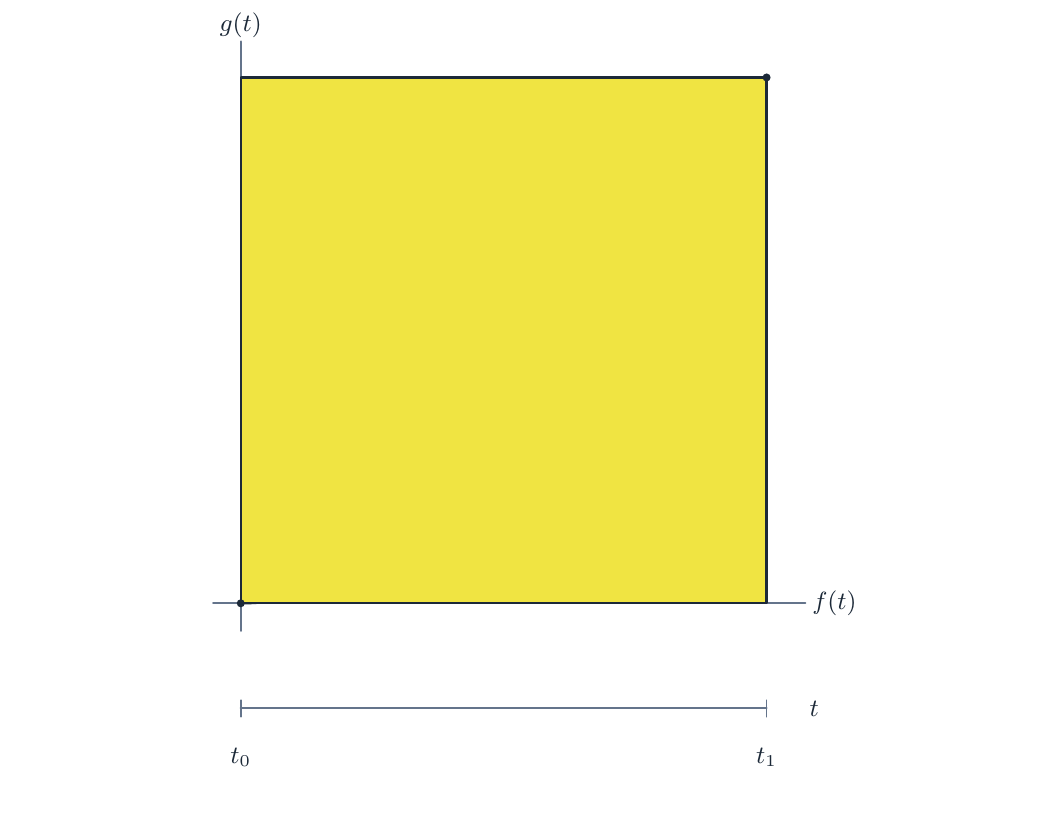
\begin{tikzpicture}[baseline=(current bounding box.north),x=1pt,y=1pt,line cap=round,line join=round]
\useasboundingbox (0,0) rectangle (360,275);
\draw[axis,line width=.75pt] (67,67) -- (281,67);
\draw[axis,line width=.75pt] (77,57) -- (77,270);
\draw[axis,line width=.75pt] (77,29) -- (267,29);
\draw[grid,line width=.3pt] (77,67) -- (77,257);
\draw[axis,line width=.55pt] (77,26) -- (77,32);
\draw[grid,line width=.3pt] (267,67) -- (267,257);
\draw[axis,line width=.55pt] (267,26) -- (267,32);
\draw[grid,line width=.3pt] (77,257) -- (267,257);
\draw[ink,line width=.85pt] plot[smooth] coordinates {(77,67) (78.9,67.019) (80.8,67.076) (82.7,67.171) (84.6,67.304) (86.5,67.475) (88.4,67.684) (90.3,67.931) (92.2,68.216) (94.1,68.539) (96,68.9) (97.9,69.299) (99.8,69.736) (101.7,70.211) (103.6,70.724) (105.5,71.275) (107.4,71.864) (109.3,72.491) (111.2,73.156) (113.1,73.859) (115,74.6) (116.9,75.379) (118.8,76.196) (120.7,77.051) (122.6,77.944) (124.5,78.875) (126.4,79.844) (128.3,80.851) (130.2,81.896) (132.1,82.979) (134,84.1) (135.9,85.259) (137.8,86.456) (139.7,87.691) (141.6,88.964) (143.5,90.275) (145.4,91.624) (147.3,93.011) (149.2,94.436) (151.1,95.899) (153,97.4) (154.9,98.939) (156.8,100.516) (158.7,102.131) (160.6,103.784) (162.5,105.475) (164.4,107.204) (166.3,108.971) (168.2,110.776) (170.1,112.619) (172,114.5) (173.9,116.419) (175.8,118.376) (177.7,120.371) (179.6,122.404) (181.5,124.475) (183.4,126.584) (185.3,128.731) (187.2,130.916) (189.1,133.139) (191,135.4) (192.9,137.699) (194.8,140.036) (196.7,142.411) (198.6,144.824) (200.5,147.275) (202.4,149.764) (204.3,152.291) (206.2,154.856) (208.1,157.459) (210,160.1) (211.9,162.779) (213.8,165.496) (215.7,168.251) (217.6,171.044) (219.5,173.875) (221.4,176.744) (223.3,179.651) (225.2,182.596) (227.1,185.579) (229,188.6) (230.9,191.659) (232.8,194.756) (234.7,197.891) (236.6,201.064) (238.5,204.275) (240.4,207.524) (242.3,210.811) (244.2,214.136) (246.1,217.499) (248,220.9) (249.9,224.339) (251.8,227.816) (253.7,231.331) (255.6,234.884) (257.5,238.475) (259.4,242.104) (261.3,245.771) (263.2,249.476) (265.1,253.219) (267,257)};
\path[fill=sharedfill,fill opacity=.85,draw=shared,draw opacity=.8,line width=.3pt] (77,67) rectangle (267,67);
\path[fill=sharedfill,fill opacity=.85,draw=shared,draw opacity=.8,line width=.3pt] (77,67) rectangle (77,257);
\path[fill=gapfill,draw=gap,draw opacity=.8,line width=.4pt] (77,67) rectangle (267,257);
\draw[ink,line width=.8pt] plot coordinates {(77,67) (267,67) (267,257)};
\draw[ink,line width=.8pt] plot coordinates {(77,67) (77,257) (267,257)};
\fill[ink] (77,67) circle[radius=1.45pt];
\fill[ink] (267,257) circle[radius=1.45pt];
\node[font=\small,text=ink,anchor=north] at (77,18) {$t_0$};
\node[font=\small,text=ink,anchor=north] at (267,18) {$t_1$};
\node[font=\small,text=ink,anchor=west] at (279,29) {$t$};
\node[font=\small,text=ink,anchor=west] at (280,67) {$f(t)$};
\node[font=\small,text=ink,anchor=south] at (77,268) {$g(t)$};
\end{tikzpicture}
\end{document}
